\chapter{Planos}

\section{Plano de ubicación general de la red}
El plano de ubicación general presenta la localización del pabellón dentro de la Ciudad Universitaria de Perayoc y la referencia vial inmediata. Sobre la imagen satelital se identifica el acceso principal, la orientación norte, el perímetro de la facultad y la ubicación aproximada del gabinete principal (MDF) respecto a los ambientes administrativos.\\
Asimismo, se señala el trazado general de las canalizaciones principales y el recorrido del backbone 
entre niveles, con una leyenda de simbología para rutas de cableado, registros y puntos de concentración. 
Esta vista sirve como base para correlacionar los planos de planta con la distribución física de la 
infraestructura de telecomunicaciones.\\
Vista desde arriba (Google Maps).\\
\begin{figure}[H]
    \centering
    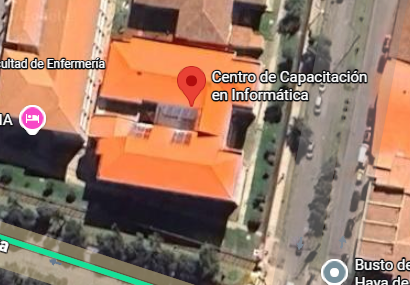
\includegraphics[width=0.7\textwidth]{GoogleMapsInformatica.png}
    \caption{Ubicación de la Facultad de Ingeniería Eléctrica, Electrónica, Informática y Mecánica de la UNSAAC. Av. De la Cultura, Nro. 733, Cusco -- Perú.}
    \label{fig:ubicacion-informatica-unsaac}
\end{figure}

\section{Planos de red, racks y telecomunicaciones}
En esta sección se presentan los planos arquitectónicos base y
las láminas de intervención y mantenimiento correspondientes a
los diferentes niveles del pabellón de Informática de la UNSAAC,
así como la organización de los gabinetes de telecomunicaciones,
patch panels y racks. Los planos detallan la ubicación de los
puntos de red, el trazado de canalizaciones, la distribución de
la infraestructura de telecomunicaciones y la disposición de los
equipos en las salas técnicas y armarios de telecomunicaciones
(MDF e IDF).

% =========================================================
% TERCER PISO
% =========================================================

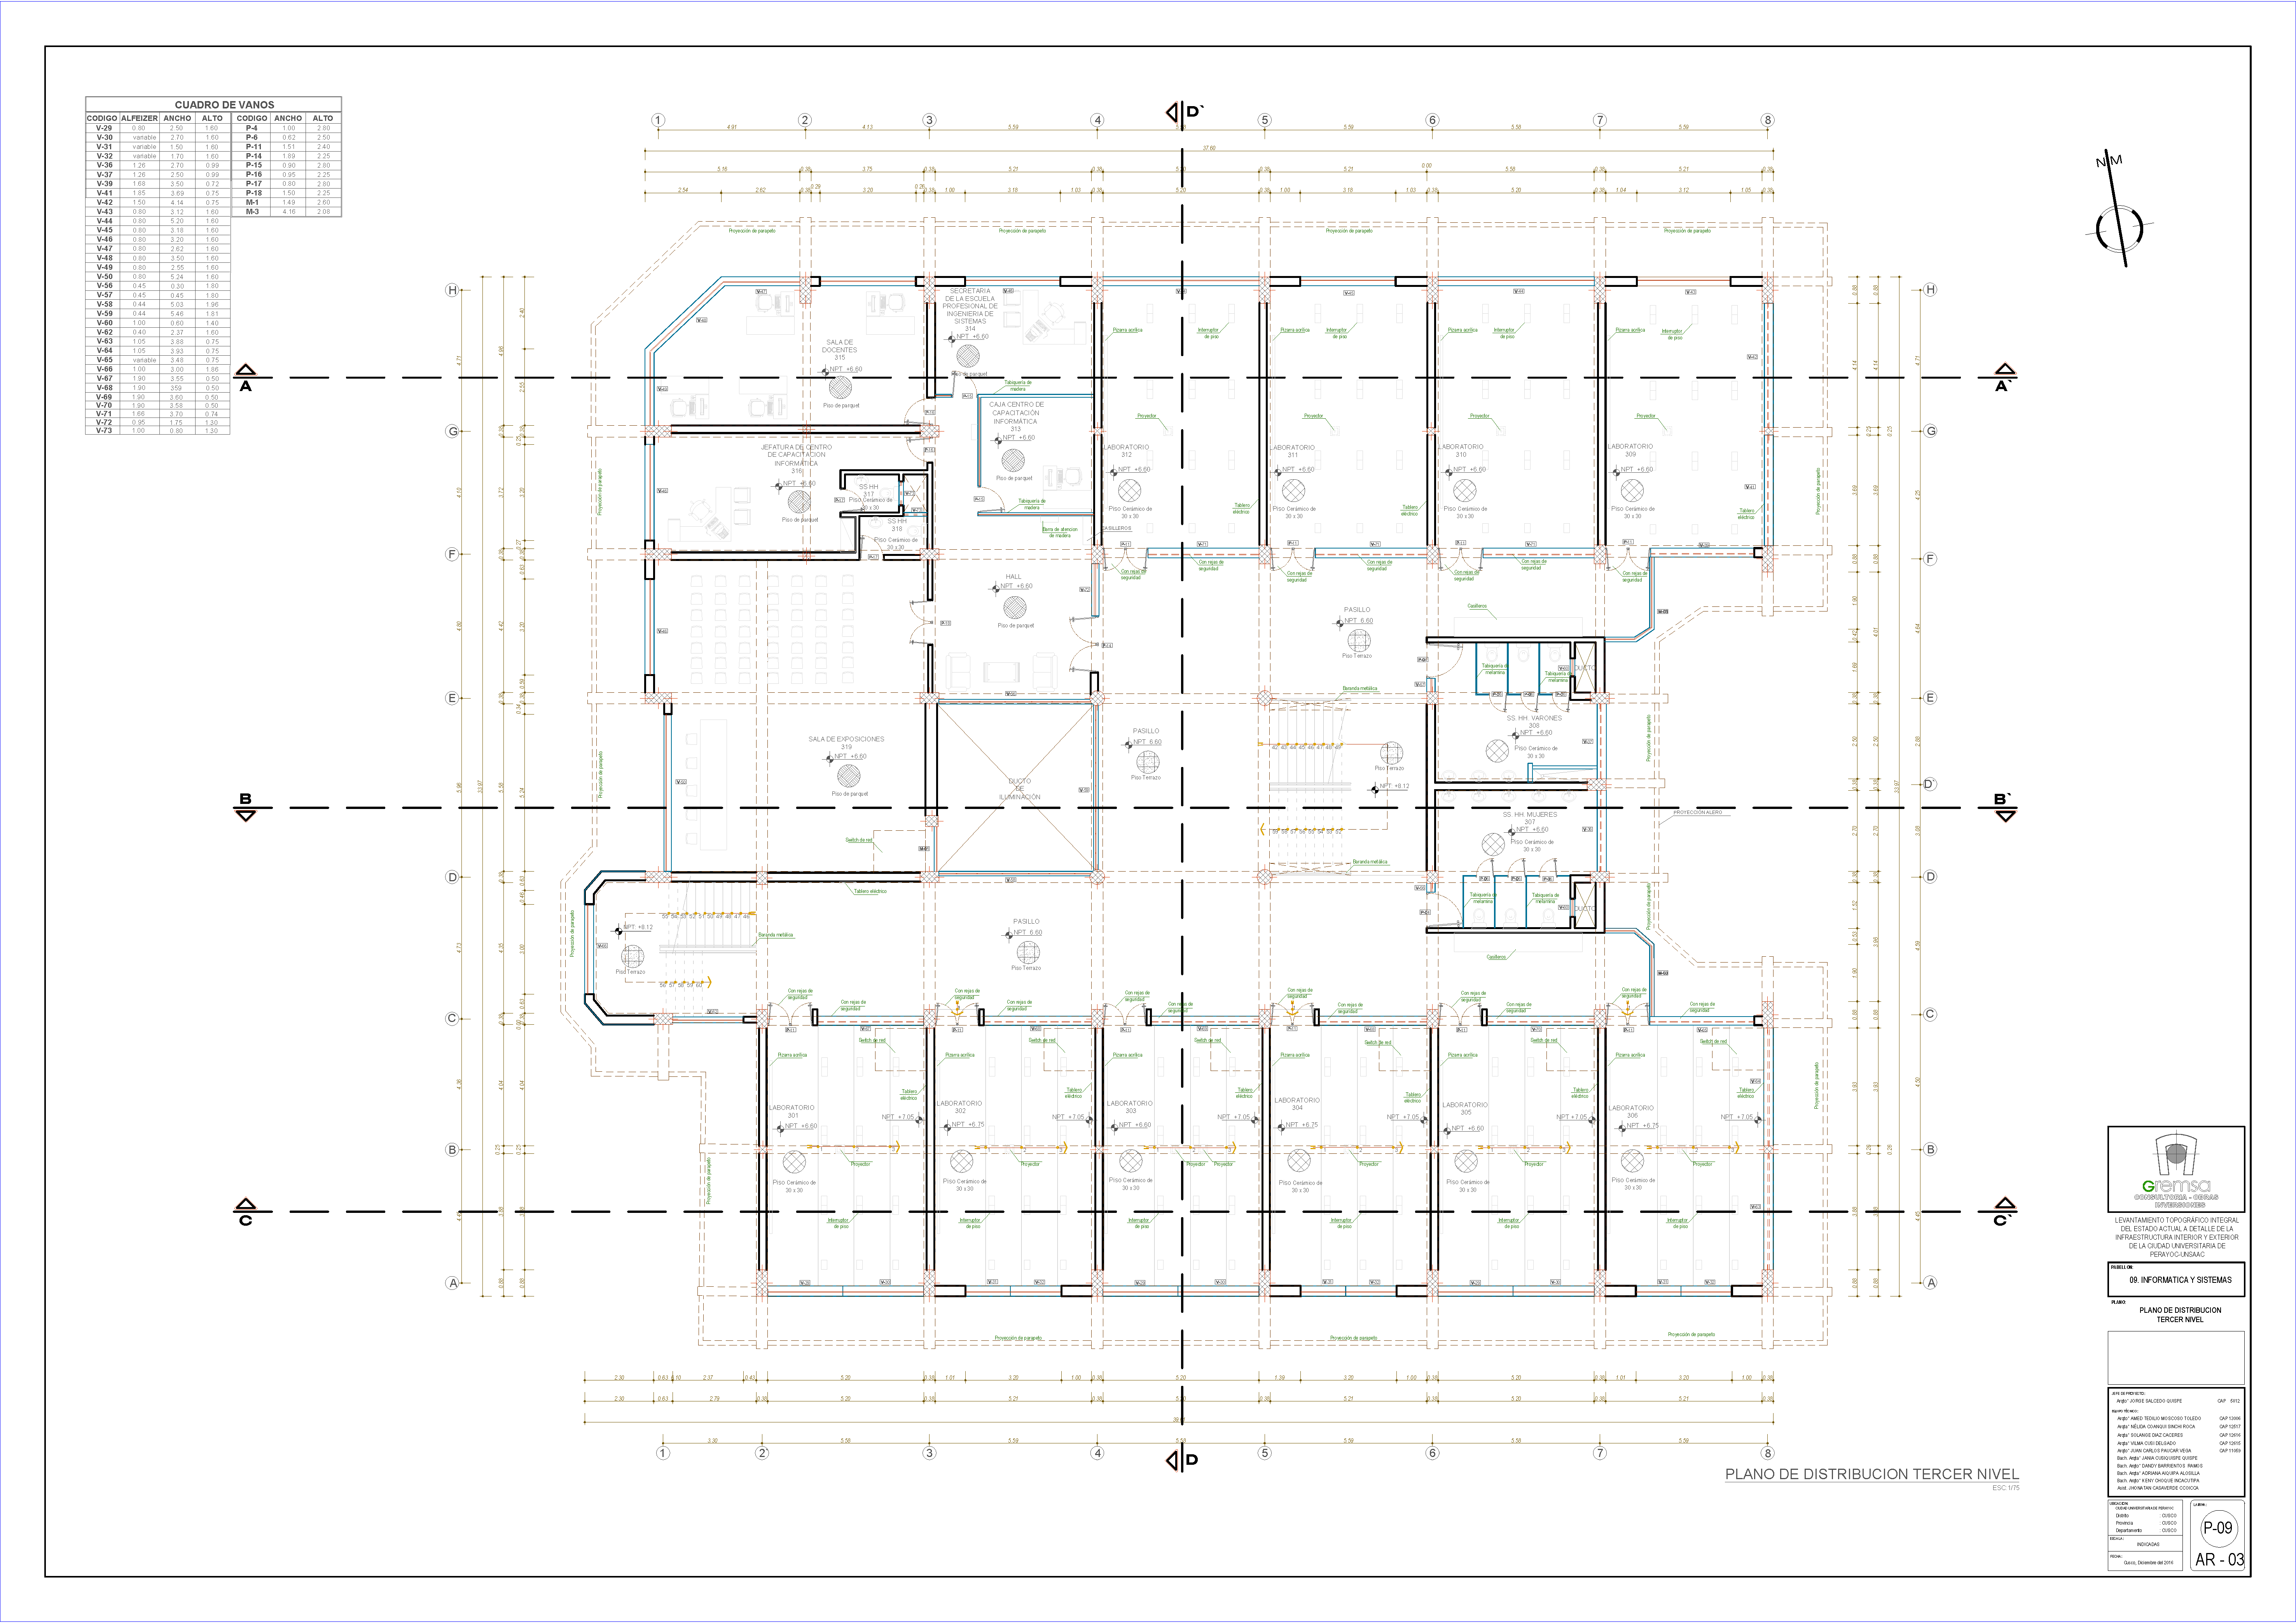
\includepdf[
    pages=1,
    landscape=true,
    scale=0.85,
    pagecommand={
        \section*{Tercer piso -- Plano base (Informatica 3er piso)}
        \thispagestyle{plain}
    }
]{Planos/INFORMATICA_3erPISO.pdf}

% =========================================================
% CUARTO PISO
% =========================================================

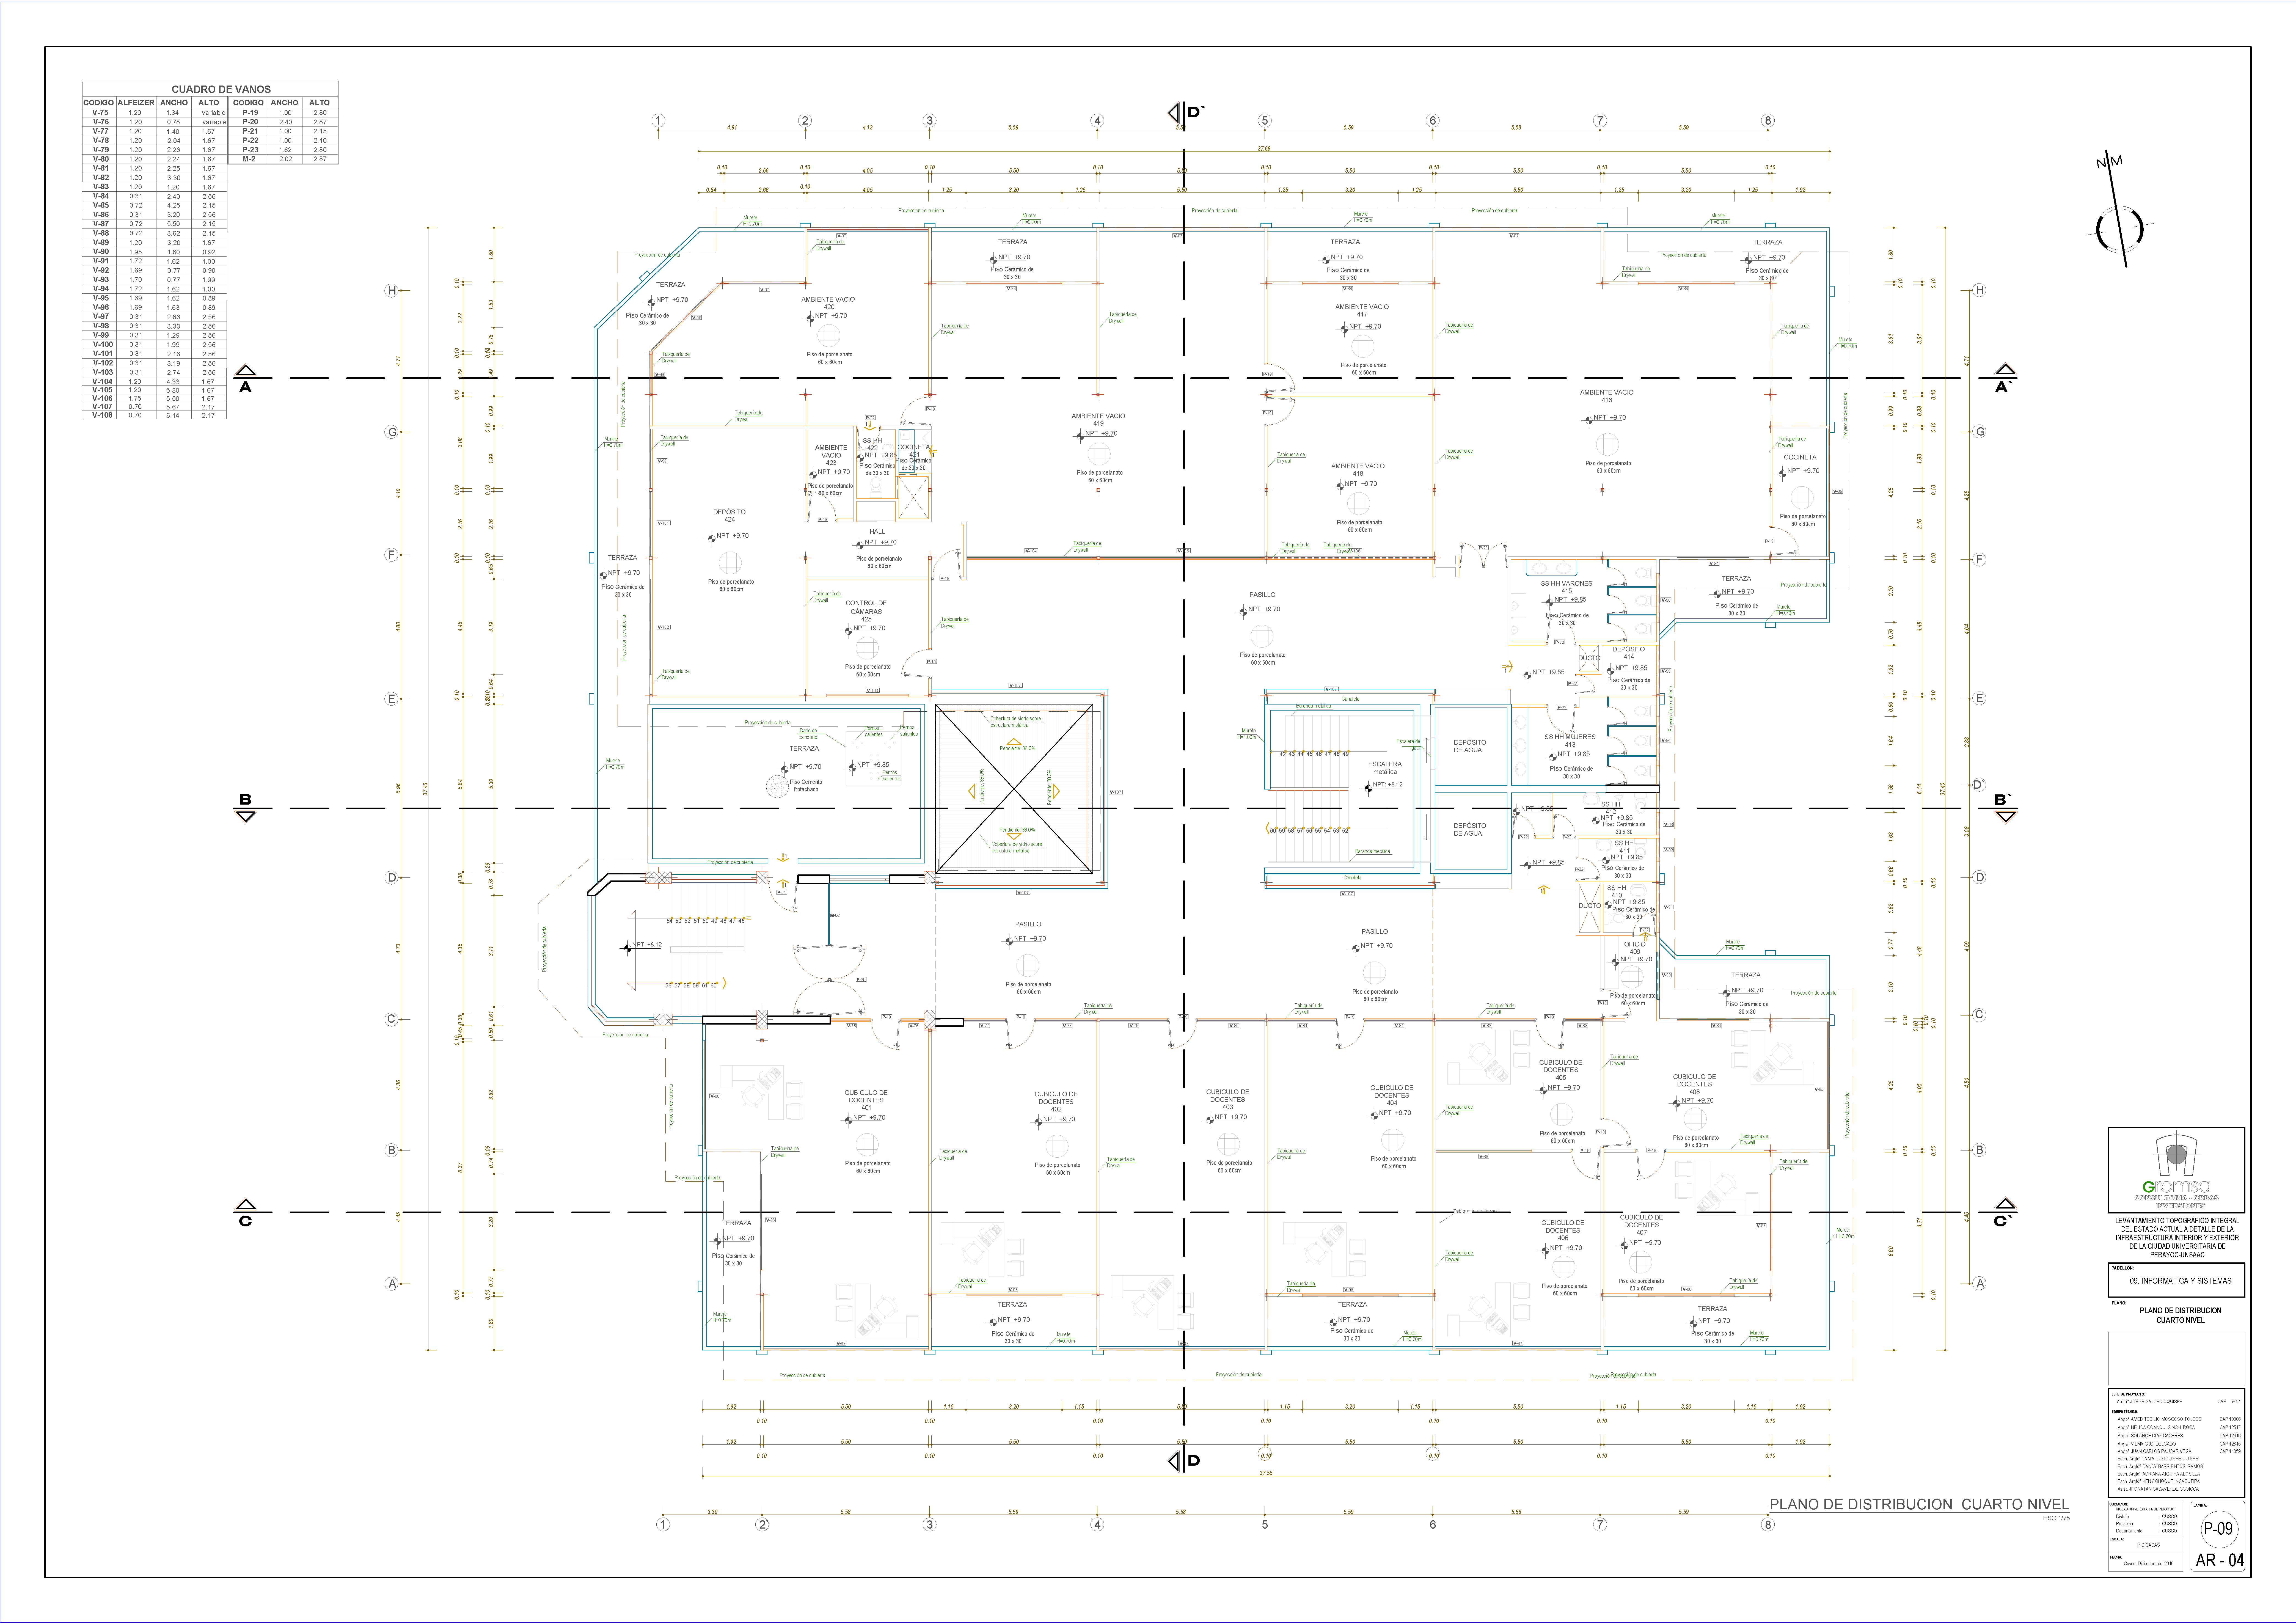
\includepdf[
    pages=1,
    landscape=true,
    scale=0.85,
    pagecommand={
        \section*{Cuarto piso -- Plano base (Informatica 4to piso)}
        \thispagestyle{plain}
    }
]{Planos/INFORMATICA_4toPISO.pdf}

% =========================================================
% TECHO
% =========================================================

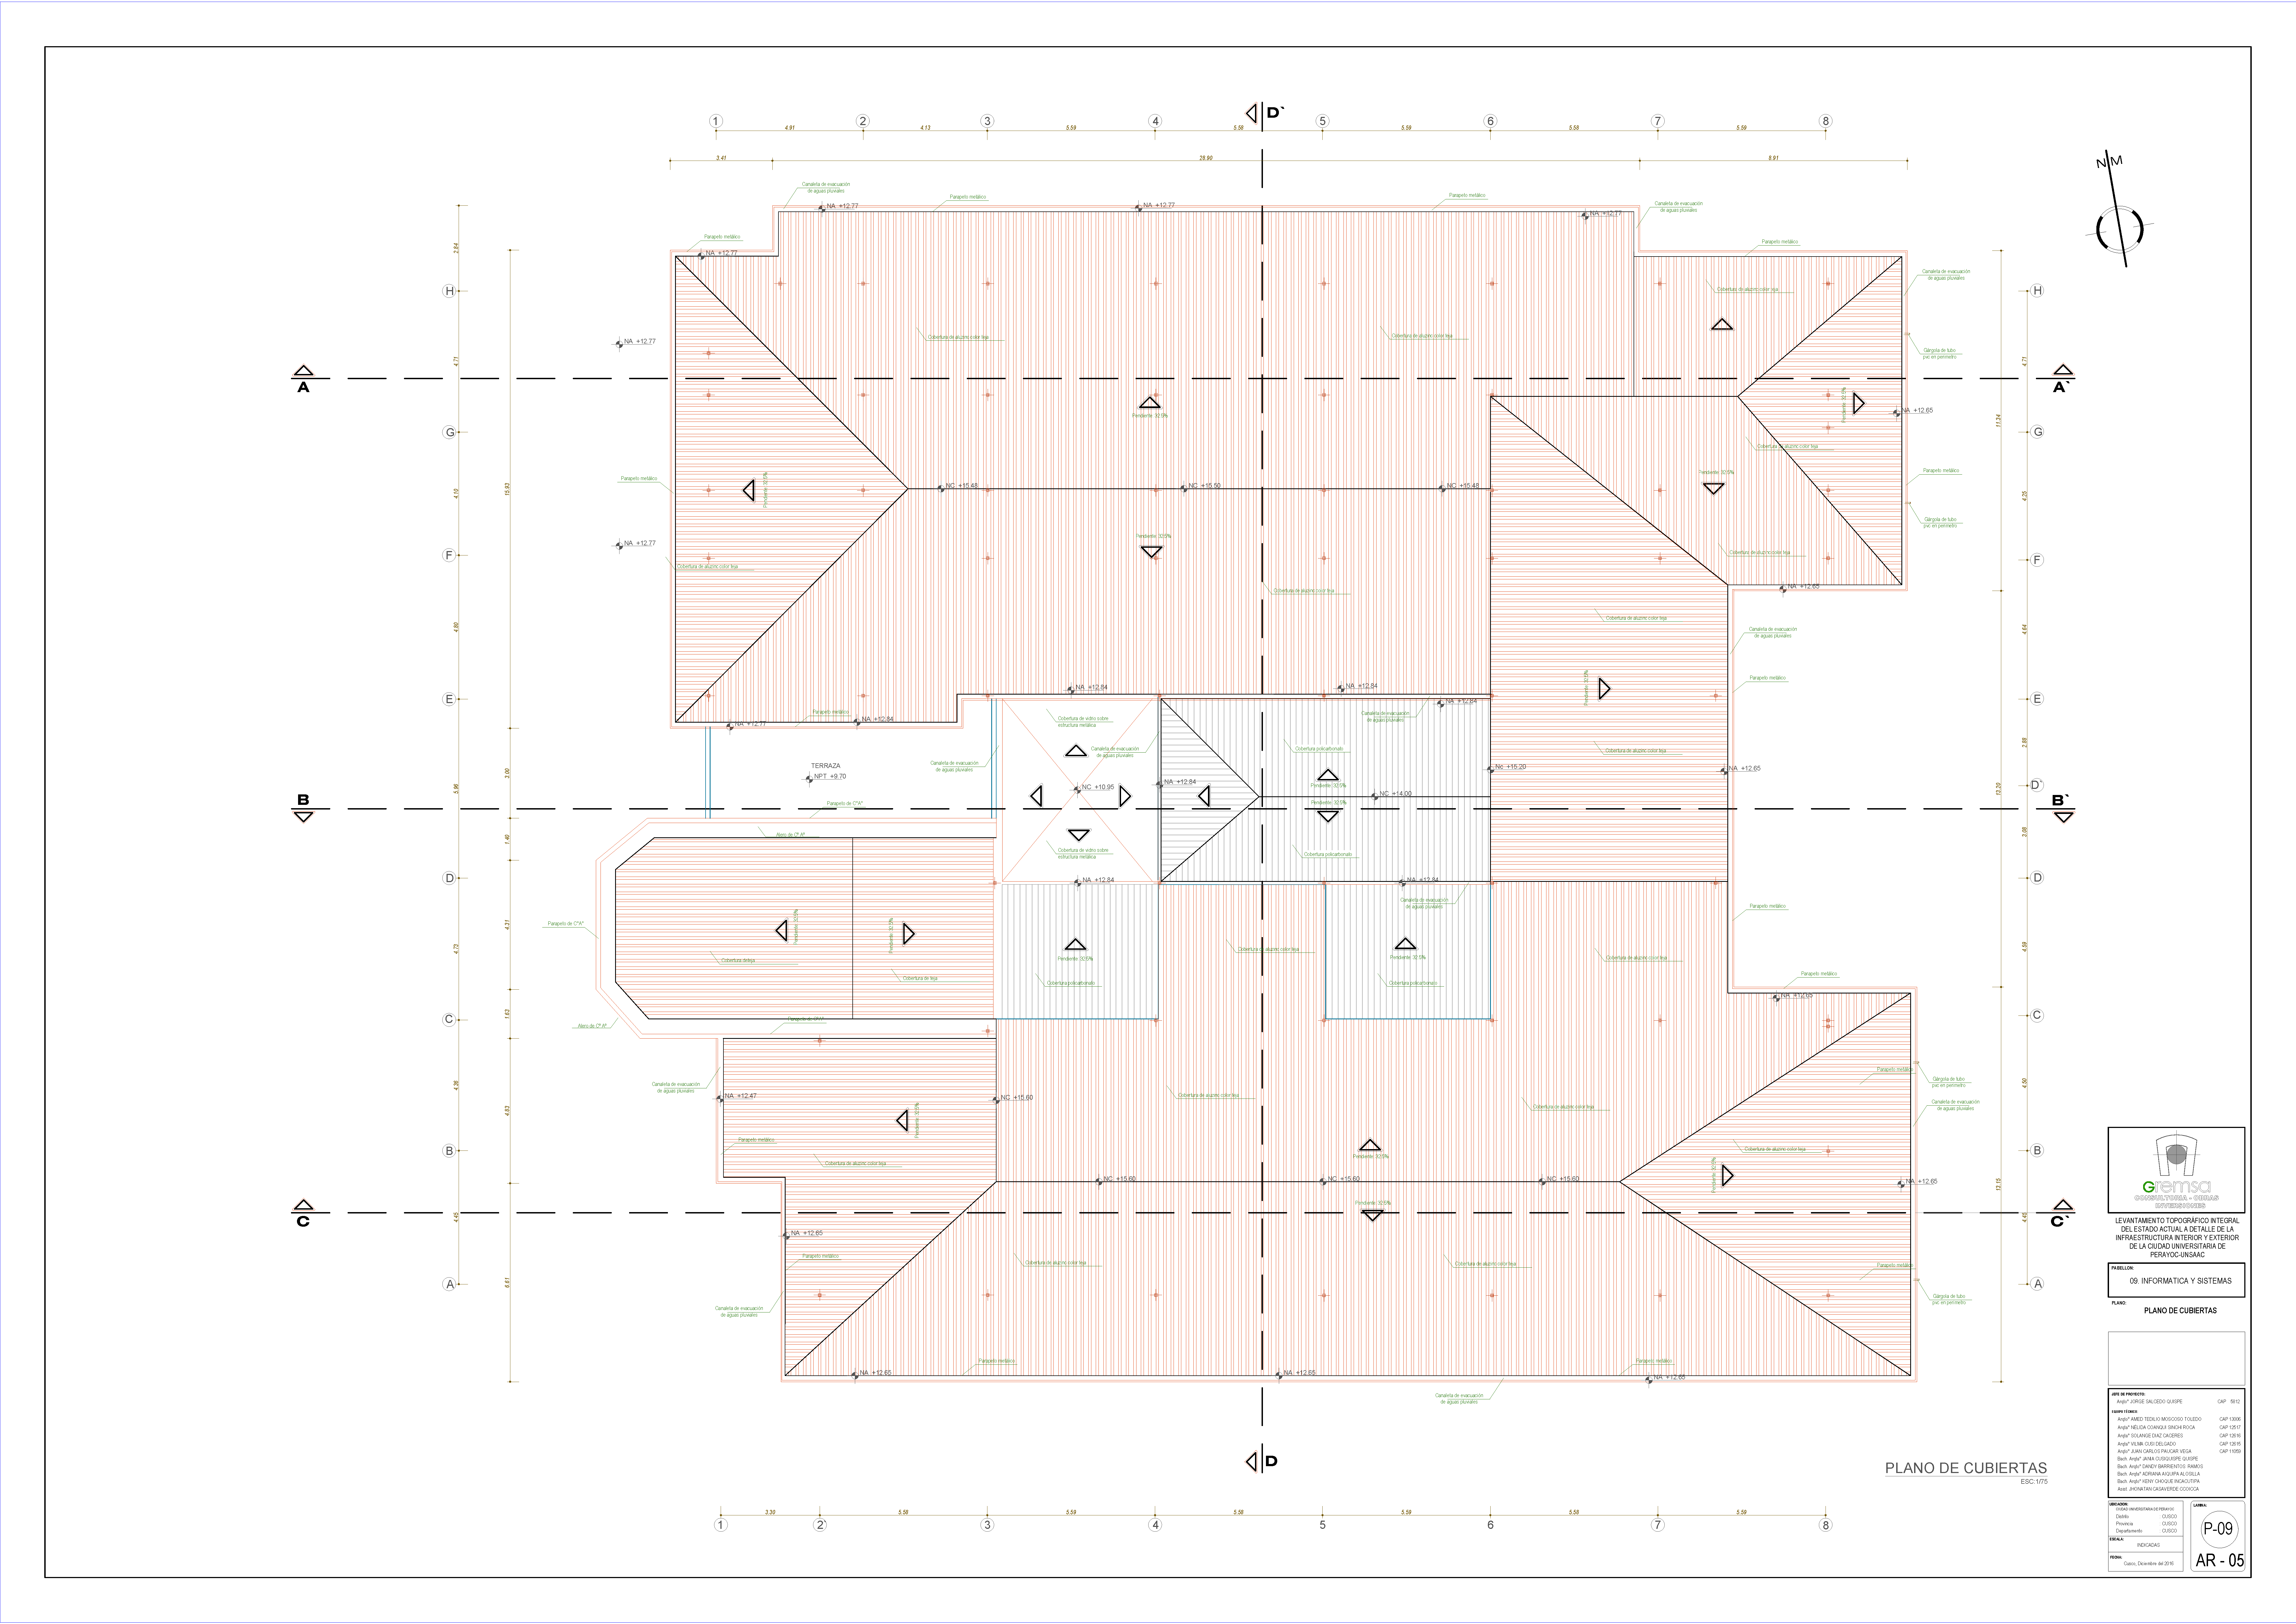
\includepdf[
    pages=1,
    landscape=true,
    scale=0.85,
    pagecommand={
        \section*{Techo -- Plano base (Informatica techo)}
        \thispagestyle{plain}
    }
]{Planos/INFORMATICA_TECHO.pdf}

% =========================================================
% TERCER PISO - Modificado
% =========================================================
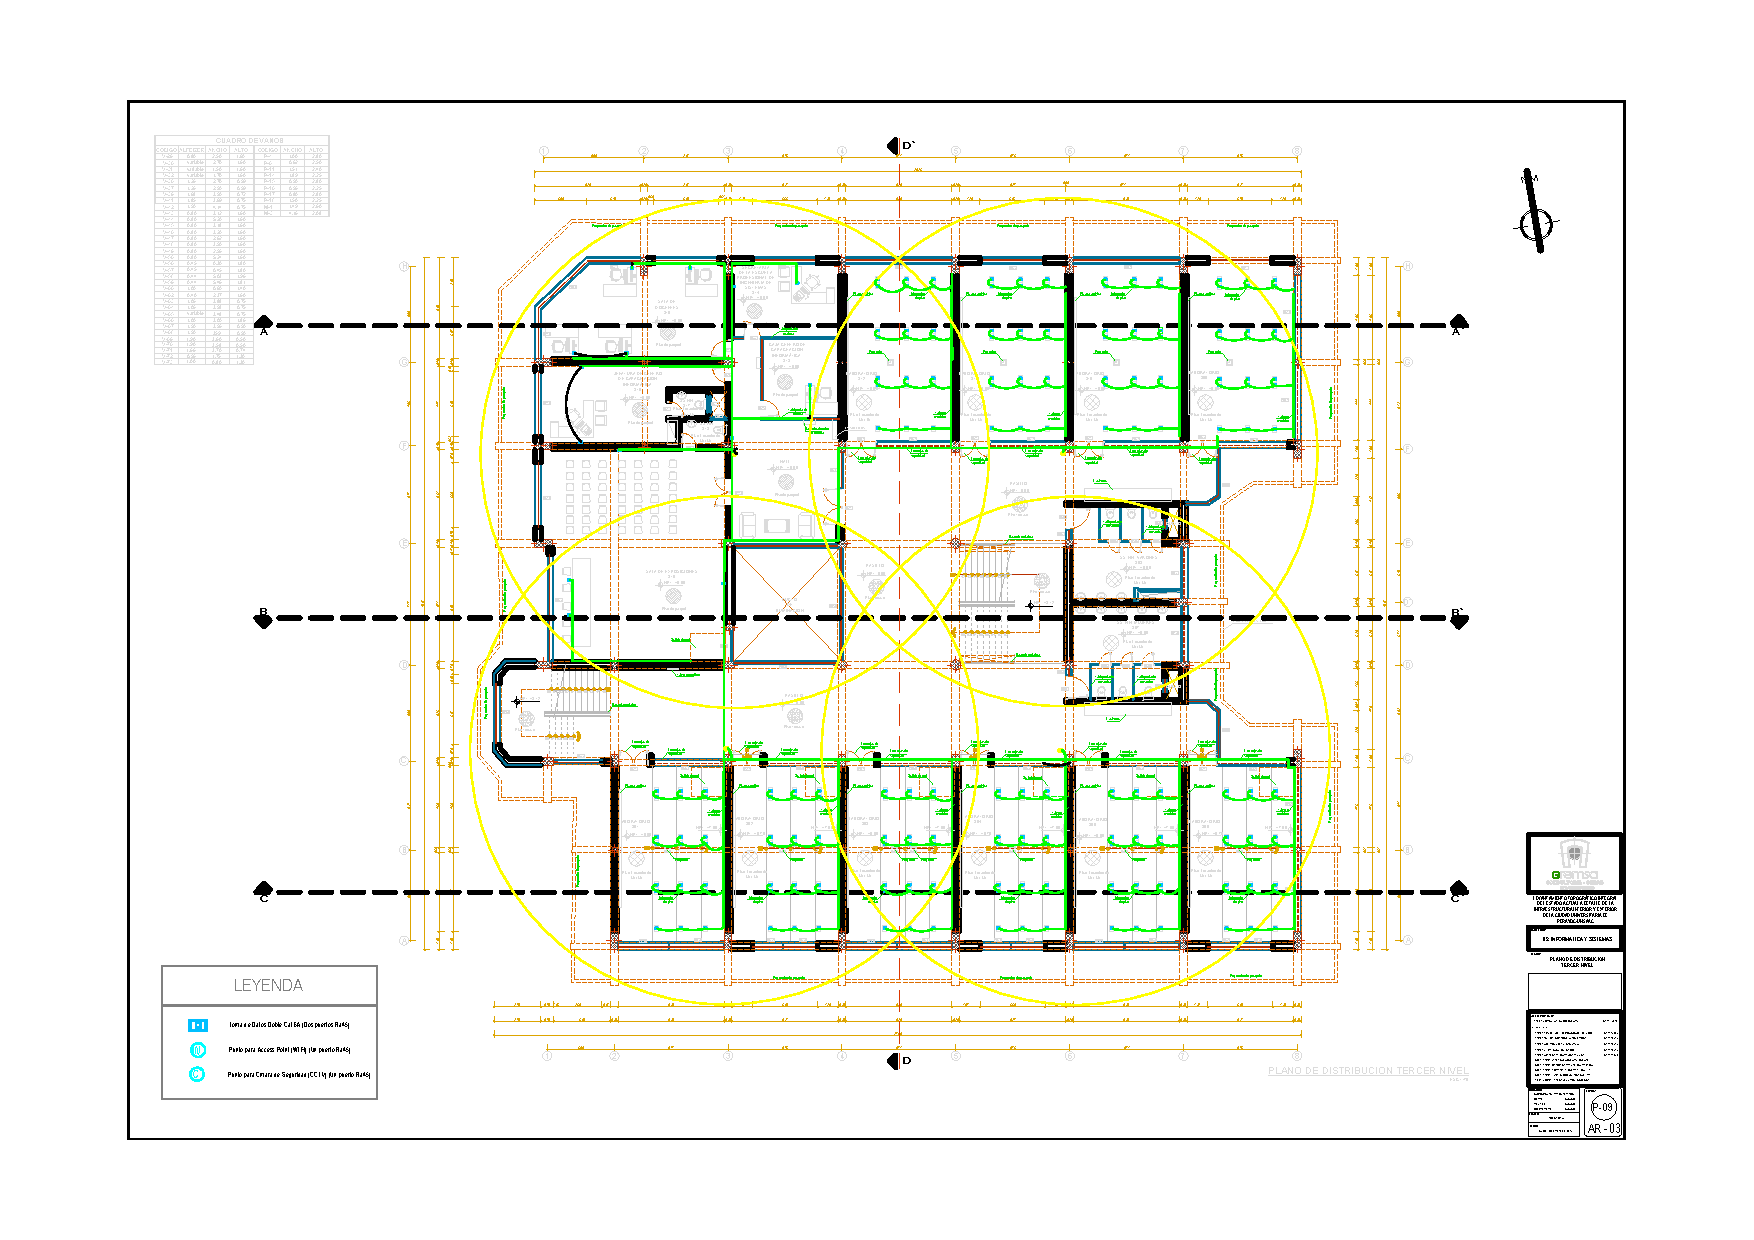
\includepdf[
    pages=1,
    landscape=true,
    scale=0.85,
    pagecommand={
        \section*{Tercer piso -- Plano Modificado (Informatica 3er piso)}
        \thispagestyle{plain}
    }
]{Planos/INFORMATICA_3erPISO_MODIFICADO.pdf}

% =========================================================
% CUARTO PISO - Modificado
% =========================================================
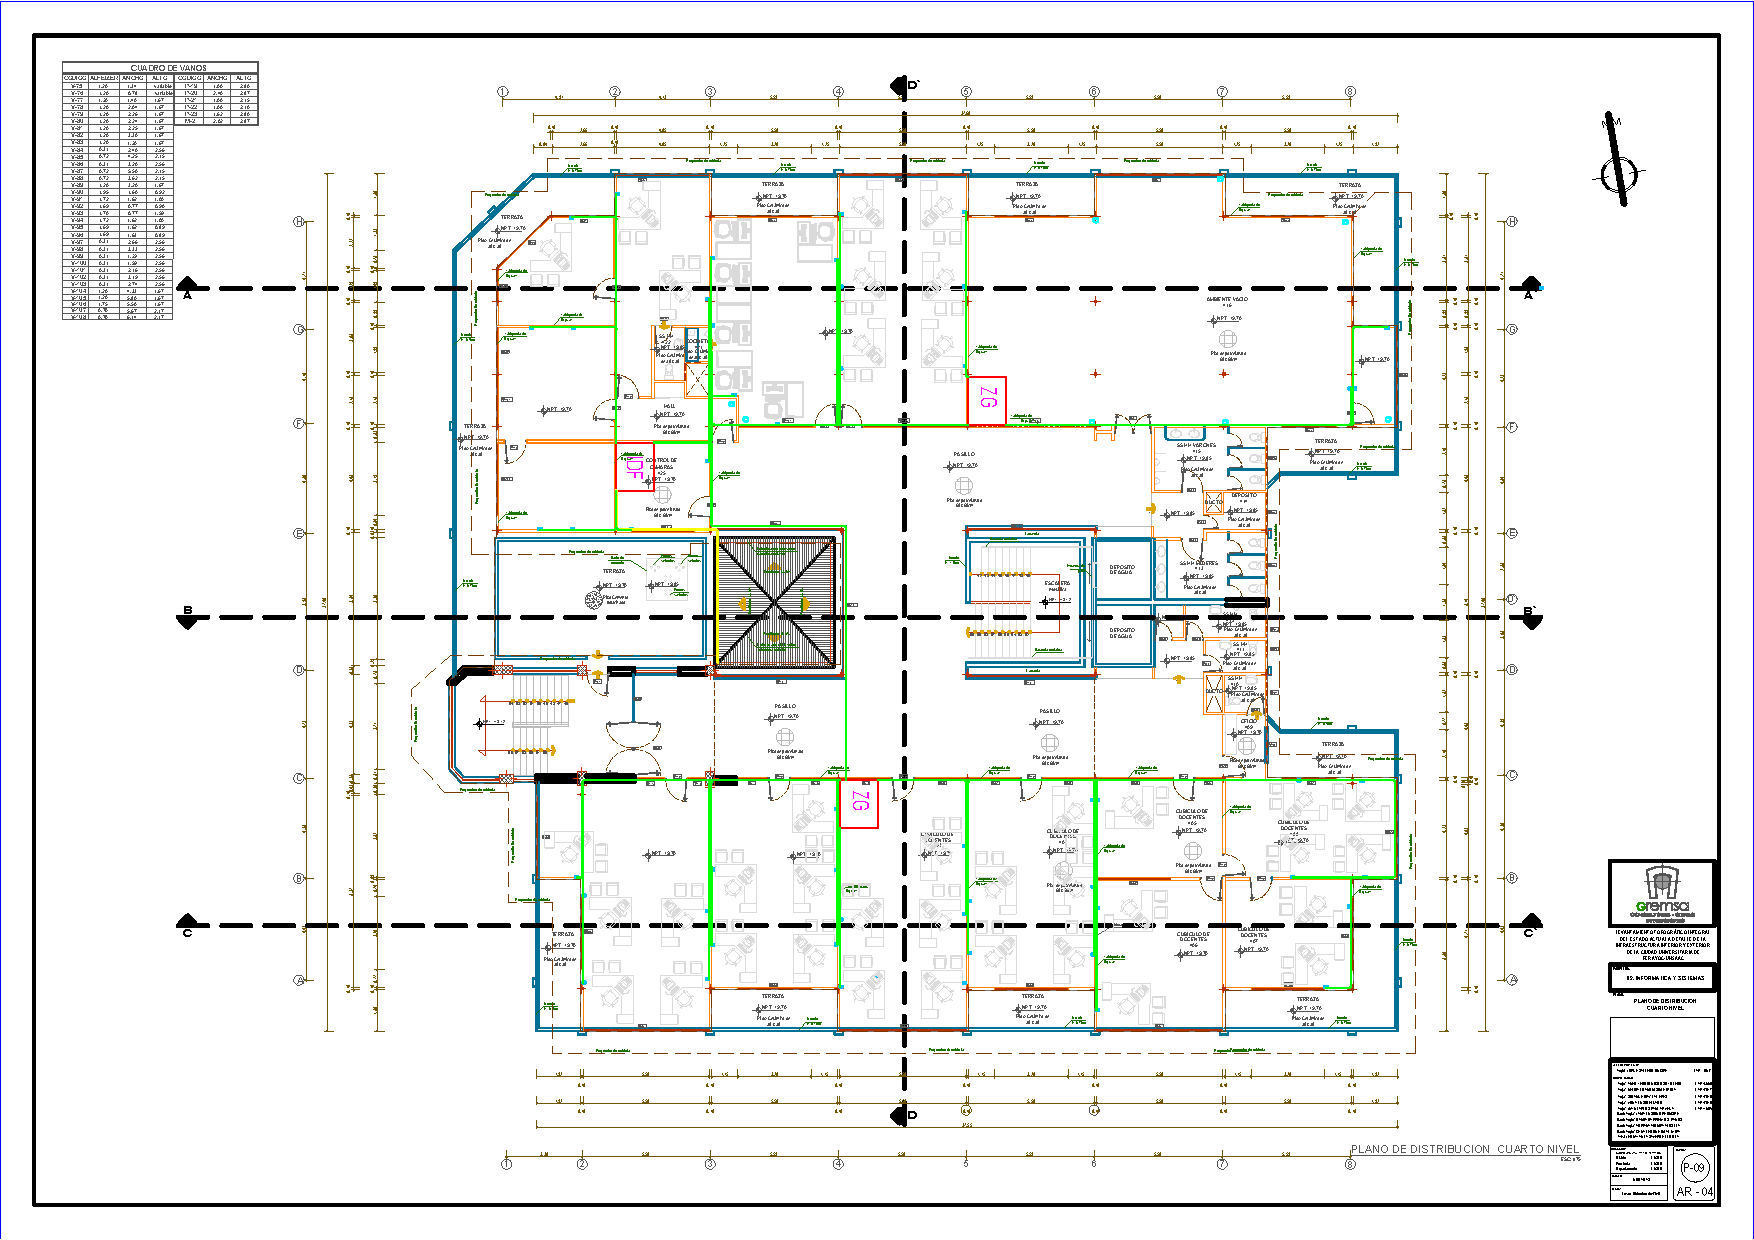
\includepdf[
    pages=1,
    landscape=true,
    scale=0.85,
    pagecommand={
        \section*{Cuarto piso -- Plano Modificado (Informatica 4to piso)}
        \thispagestyle{plain}
    }
]{Planos/INFORMATICA_4toPISO_MODIFICADO.pdf}



\section{Plano de backbone}
Interconexión de armarios principales y secundarios.

\section{Detalles constructivos de ductos, bandejas y registros}
Ductería, bandejas, registros, puesta a tierra.

\section{Diagrama de puesta a tierra}